\section{What Makes a Neuron Fire?}
\label{sec:what-makes-a-neuron-fire}

\begin{rem}
  Response tuning curves characterize the average response of a neuron to a given stimulus. We now consider the complementary procedure of averaging the stimuli that produce a given response.  
\end{rem}
\begin{rem}
  To average stimuli in this way, we need to specify what fixed response we will use to “trigger” the average. The most obvious choice is the firing of an action potential. Thus, we ask, “What, on average, did the stimulus do before an action potential was fired?” The resulting quantity, called the spike-triggered average stimulus, provides a useful way of characterizing neuronal selectivity.
  %Spike-triggered averages are computed using stimuli characterized by a parameter $s(t)$ that varies over time. 
\end{rem}

\subsection{Describing the Stimulus}
\begin{ntn}
  \label{defn:noticeable difference}
  Weber measured how different the intensity of two stimuli had to be for them to be reliably discriminated, the “just noticeable” difference $\Delta{s}$.  
\end{ntn}
\begin{prin}[Weber's law]
  \label{prin:Weber's law}
  $\Delta{s}$ is proportional to the magnitude of the stimulus $s$, so that $\Delta{s}/s$ is constant for a given stimulus.
\end{prin}

\begin{rem}
  Fechner suggested that noticeable differences set the scale for perceived stimulus intensities.% in Principle \ref{prin:Fechner's law}
\end{rem}

\begin{prin}[Fechner's law]
  \label{prin:Fechner's law}
  Integrating Weber's law, the perceived intensity of a stimulus of absolute intensity $s$ varies as $\log{s}$.
\end{prin}

\begin{exm}
  \label{exm:Steady-state responses}
  %Neurons responding to sensory stimuli face the difficult task of encoding parameters that can vary over an enormous dynamic range. For example, photoreceptors in the retina can respond to single photons or can operate in bright light with an influx of millions of photons per second.
  To deal with such wide-ranging 
  stimuli, sensory neurons often respond most strongly to rapid changes in stimulus properties and are relatively insensitive to steady-state levels. Steady-state responses are highly compressed functions of stimulus intensity, typically with logarithmic or weak power-law dependences. This compression has an interesting psychophysical correlate.
  %in Principle \ref{prin:Weber's law} and Principle \ref{prin:Fechner's law}.
\end{exm}

\begin{rem}
  Sensory systems make numerous adaptations, using a variety of mechanisms, to adjust to the average level of stimulus intensity. When a stimulus generates such adaptation, the relationship between stimulus and response is often studied in a potentially simpler regime by describing responses to fluctuations about a mean stimulus level. 
\end{rem}

\begin{asm}
  \label{defn:impose-s(t)-condition}
  We frequently impose this condition that $s(t)$ satisfies
  \begin{displaymath}
    \frac{1}{T}\int_0^T s(t) dt = 0,
  \end{displaymath}
  that is, $s(t)$'s time average over the duration of a trial is 0.
\end{asm}


\begin{rem}
   Our analysis of neural encoding involves two different types of averages: averages over repeated trials that employ the same stimulus, which we denote by angle brackets, and averages over different stimuli. We could introduce a second notation for averages over stimuli, but this can be avoided when using time-dependent stimuli.
\end{rem}
\begin{defn}[Stimulus and time averages]
  \label{defn:stimulus and time averages}
  Instead of presenting a number of different stimuli and averaging over them, we can string together all of the stimuli we wish to consider into a single time-dependent stimulus sequence and average over time. Thus, stimulus averages are replaced by \emph{time averages}.  
\end{defn}

% \begin{rem}
%   Although a response recorded over a trial depends only on the values taken by $s(t)$ during that trial, some of 
%   the mathematical analyses presented in this chapter and in chapter \ref{cha:Neural Encoding II} are simplified if we define the stimulus 
%   at other times as well.
% \end{rem}

\begin{prop}[Periodic stimulus]
  If integrals involving the stimulus are time-translationally invariant,
  then for any function $h$ and time interval $\tau $
  \begin{equation}
    \label{equ:1.18}
    \int_0^T h(s(t+\tau)) dt = \int_{\tau}^{T+\tau} h(s(t)) dt = \int_0^T h(s(t)) dt.
  \end{equation}
  To assure the last equality, we define the stimulus outside the time limits of the trial by the relation 
  $s(T+\tau) = s(\tau)$ for any $\tau$, thereby making the stimulus periodic.
\end{prop}

\subsection{The Spike-Triggered Average}
\begin{defn}
  \label{defn:Spi-Tri Ave}
  \emph{The spike-triggered average} stimulus, $C(\tau)$, is the average value of the stimulus $s$ a time interval $\tau$ 
  before a spike is fired. The \emph{spike-triggered average} $C(\tau)$ is a number of the form
  \begin{equation}
    \label{equ:1.19}
    C(\tau) = \left \langle \frac{1}{n} \sum_{i=1}^{n} s(t_i - \tau) \right \rangle \approx \frac{1}{\langle n \rangle} \left \langle \sum_{i=1}^n s(t_i - \tau) \right \rangle,
  \end{equation}
  where $n$ is the total number of spikes on each trial and $t_i$ is the time when the spike occurrs for $i = 1, 2, \cdots, n$.  If $n$ is large, it is well approximated by $\langle n \rangle$.
\end{defn}

% \begin{rem}
%   In Definition \ref{defn:Spi-Tri Ave}, the approximate equality of the last expression follows from the fact that if n is large, the total number of 
%   spikes on each trial is well approximated by the average number of spikes per trial, $n \approx \langle n \rangle$.
% \end{rem}
% \begin{rem}
%   For a spike occurring at time $t_i$, we determine $s(t_i - \tau)$,
%   and then we sum over all $n$ spikes in a trial, $i = 1, 2, \cdots, n$, and divide the total by $n$.
%   In addition, we average over trials.
% \end{rem}

\begin{rem}
   We make use of this approximation in Equation \ref{equ:1.19} because it allows us to relate the spike-triggered average to other 
   quantities commonly used to characterize the relationship between stimulus and response (see Proposition \ref{prop:integral-STAS}).
\end{rem}

\begin{exm}
 %  \begin{figure}[H]
%   \centering
%   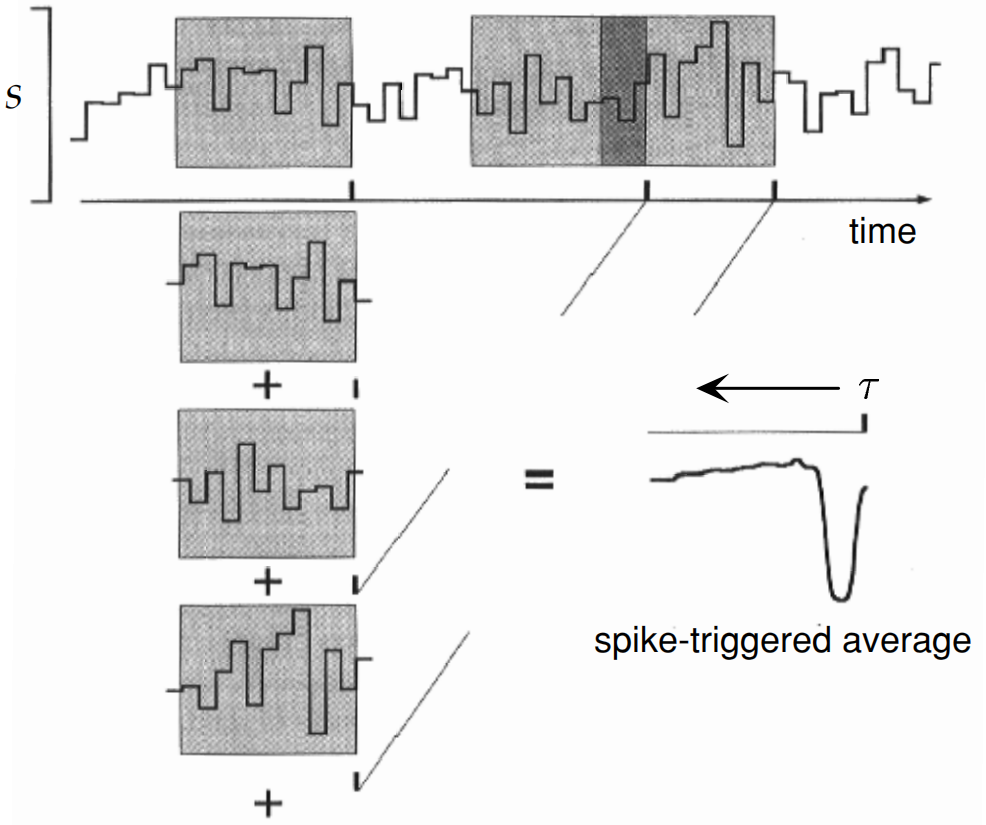
\includegraphics[scale=0.50]{./png/computation-spiTriAvST.png}
%   \caption{Schematic of the procedure for computing the spike-triggered average stimulus. Each gray rectangle contains the stimulus prior to one of the spikes shown along the time axis. These are averaged to produce the waveform shown at the lower right, which is the average stimulus before a spike. The stimulus in this example is a piecewise constant function of time. (Adapted from Rieke et al.,1997.)}
%   \label{fig1.8:computation-spiTriAvSt}  
% \end{figure}
% % \newpage
  \label{exm:compute-SpiTriAve}
  %Figure \ref{fig:1.8}
  The following figure provides a schematic description of the computation of the spike-triggered average. Each time a 
  spike appears, the stimulus in a time window preceding the spike is recorded. Although the range of $\tau$ 
  values in Equation \ref{equ:1.19} is unlimited, the response is typically affected only by the stimulus in a window 
  a few hundred milliseconds wide immediately preceding a spike. More precisely, we expect $C(\tau)$ to approach $0$ 
  for positive $\tau$ values larger than the correlation time between the stimulus and the response. If the 
  stimulus has no temporal correlations with itself, we also expect $C(\tau)$ to be $0$ for $\tau < 0$, because 
  the response of a neuron cannot depend on future stimuli. In practice, the stimulus is recorded only over a 
  finite time period, as indicated by the shaded areas in the figure below.
  % figure \ref{fig:1.8}.
  The recorded stimuli for all 
  spikes are then summed and the procedure is repeated over multiple trials.
\end{exm}
\begin{center}
  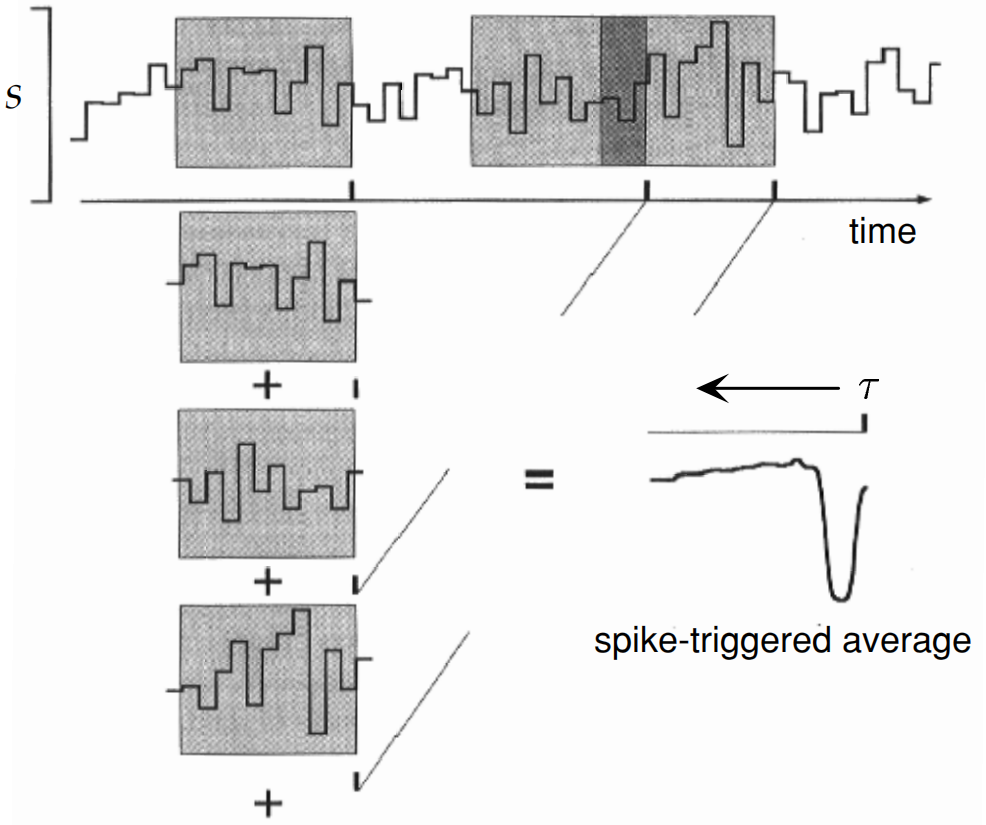
\includegraphics[scale=0.46]{./png/computation-spiTriAvST.png}
  %figurecaption{Schematic of the procedure for computing the spike-triggered average stimulus. Each gray rectangle contains the stimulus prior to one of the spikes shown along the time axis. These are averaged to produce the waveform shown at the lower right, which is the average stimulus before a spike. The stimulus in this example is a piecewise constant function of time. (Adapted from Rieke et al.,1997.)}
  \label{fig:1.8}  
\end{center}

\begin{prop}
  \label{prop:integral-STAS}
  The spike-triggered average stimulus can be expressed as an integral of the stimulus times the neural response function of Equation \ref{equ:1.1}. If we replace the sum over spikes with an integral, as in Equation \ref{equ:1.2}, and use the approximate expression for $C(\tau)$ in Equation \ref{equ:1.19}, we find
  \begin{equation}
    \label{equ:1.20}
    C(\tau) = \frac{1}{\lrangle{n}} \int_0^T \lrangle{\rho(t)}s(t-\tau) dt = \frac{1}{\lrangle{n}} \int_0^T \text{r}(t) s(t-\tau) dt.
  \end{equation}
  The second equality is due to the equivalence of $\lrangle{\rho(t)}$ and $\text{r}(t)$ within integrals. Equation \ref{equ:1.20} allows us to relate the spike-triggered average to the correlation function of the firing rate and the stimulus.
\end{prop}

\begin{defn}
  \label{defn:col-func}
  The correlation function of the continuous functions $f$ and $g$ on $[0, T]$ is
  \begin{equation}
    \label{equ:1.21}
    R(\tau) = \frac{1}{T} \int_0^T f(t) g(t+\tau) dt.
  \end{equation}
\end{defn}
\begin{prop}
  \label{defn:Qrs}
  The correlation function of the firing rate and the stimulus (also called \emph{firing-rate stimulus correlation function}) is
  \begin{equation}
    \label{equ:1.21}
    Q_{\text{r}s} = \frac{1}{T} \int_0^T \text{r}(t) s(t+\tau) dt.
  \end{equation}
\end{prop}
\begin{rem}
  Correlation functions are a useful way of determining how two quantities that vary over time are related to one another. The two quantities being related are evaluated at different times, one at time $t$ and the other at time $t+\tau$. The correlation function is then obtained by averaging their product over all $t$ values, and it is a function of $\tau$.
\end{rem}
\begin{prop}
  \label{prop:rCF}
  By comparing Equations \ref{equ:1.20} and \ref{equ:1.21}, we find that
  \begin{equation}
    \label{equ:1.22}
    C(\tau) = \frac{1}{\lrangle{r}} Q_{\text{r}s}(-\tau),
  \end{equation}
  where $\lrangle{r} = \lrangle{n}/T$ is the average firing rate over the set of trials.
  Because the argument of the correlation function in Equation \ref{equ:1.22} is $-\tau$, the spike-triggered average stimulus is often called \emph{the reverse correlation function}.
\end{prop}
% \begin{rem}
%    Because the argument of the correlation function in Equation \ref{equ:1.22} is $-\tau$, the spike-triggered average stimulus is often called \emph{the reverse correlation function}. It is proportional to the correlation of the firing rate with the stimulus at preceding times.
% \end{rem}

\begin{exm}
  \label{exm:spi-tri-ave in elefish}
  % Figure \ref{fig:1.9}
  The following figure shows the spike-triggered average stimulus for a neuron in the electrosensory lateral-line lobe of the weakly electric fish \emph{Eigenmannia}.
  % Weakly electric fish generate oscillating electric fields from an internal electric organ. Distortions in the electric field produced by nearby objects are detected by sensors spread over the skin of the fish. The lateral-line lobe acts as a relay station along the processing pathway for electrosensory signals.
  Fluctuating electrical potentials, such as that shown in the upper left trace of the figure below,
  % figure \ref{fig:1.9},
  elicit responses from electrosensory lateral-line lobe neurons, as seen in the lower left trace. The spike-triggered average stimulus, plotted at the right, indicates that, on average, the electric potential made a positive upswing followed by a large negative deviation prior to a spike being fired by this neuron.
\end{exm}
\begin{center}
  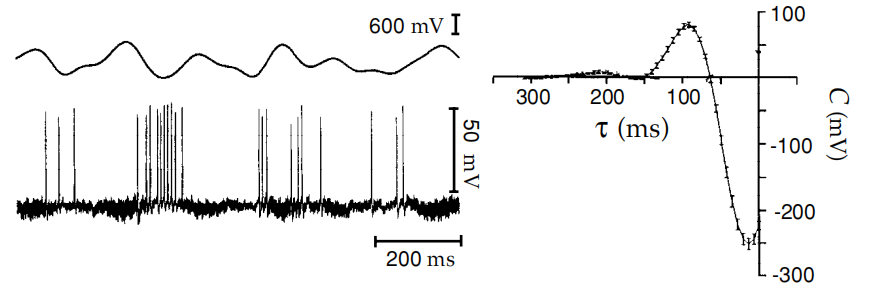
\includegraphics[scale=0.44]{./png/spiTriAvST-elefish.png}
   %figurecaption{The spike-triggered average stimulus for a neuron of the electrosensory lateral-line lobe of the weakly electric fish Eigenmannia. The upper left trace is the potential used to generate the electric field to which this neuron is sensitive. The evoked spike train is plotted below the stimulus potential. The plot on the right is the spike-triggered average stimulus. (Adapted from Gabbiani et al., 1996.)}
  \label{fig:1.9}
\end{center}

\begin{rem}
   The spike-triggered average stimulus is widely used to study and characterize neural responses. Because $C(\tau)$ is the average value of the stimulus at a time $\tau$ before a spike, larger values of $\tau$ represent times farther in the past relative to the time of the triggering spike. For this reason, we spike-triggered averages with the time axis going backward compared to the normal convention. This allows the average spike-triggering stimulus to be read off from the plots in the usual left-to-right order.
\end{rem}

\begin{rem}
  The results obtained by spike-triggered averaging depend on the particular set of stimuli used during an experiment. How should this set be chosen? In chapter \ref{cha:Neural Encoding II}, we show that there are certain advantages to using a stimulus that is uncorrelated from one time to the next, a white-noise stimulus. A heuristic argument supporting the use of such stimuli is that in asking what makes a neuron fire, we may want to sample its responses to stimulus fluctuations at all frequencies with equal weight (i.e., equal power), and this is one of the properties of white-noise stimuli. In practice, white-noise stimuli can be generated with equal power only up to a finite frequency cutoff, but neurons respond to stimulus fluctuations only within a limited frequency range anyway. 
  % Figure \ref{fig:1.9}
The figure in Example \ref{exm:spi-tri-ave in elefish} is based on such an approximate white-noise stimulus.The power in a signal as a function of its frequency is called the power spectrum or power spectral density. White noise has a flat power spectrum.
\end{rem}

\subsection{White-Noise Stimuli}
\label{sec:white-noiseStimuli}

\begin{defn}
  \label{defn:whi-noi sti}
  The defining characteristic of \emph{white-noise stimulus} is that its value at any one time is uncorrelated with its value at any other time.
\end{defn}

\begin{prop}
  \label{prop:whiteNoiseAutocorrelation}
  The stimulus-stimulus correlation function (also called the \emph{stimulus autocorrelation}) for white-noise stimulus $s(t)$ can be expressed by
  \begin{equation}
    \label{equ:1.24}
    Q_{ss}(\tau) = \sigma_s^2\delta(\tau)
  \end{equation}
  with some constant $\sigma_s$.
\end{prop}
\begin{proof}
  By Definition \ref{defn:col-func}, we have
  \begin{equation}
    \label{equ:1.23}
    Q_{ss}(\tau) = \frac{1}{T} \int_0^T s(t)s(t+\tau) dt.
  \end{equation}
  Just as a correlation function provides information about the temporal relationship between two quantities, so an autocorrelation function tells us
about how a quantity at one time is related to itself evaluated at another
time. For white noise, the stimulus autocorrelation function is 0 in the
range $-T/2 < \tau < T/2$ except when $\tau=0$, thus, over this range we have Equation \ref{equ:1.24}.
\end{proof}

\begin{defn}
  \label{defn:power-spectrum}
  The \emph{power spectrum} for a stimulus $s(t)$ is the Fourier transform of the autocorrelation function of $s(t)$.
  \begin{equation}
    \label{equ:1.40}
    \widetilde{Q}_{ss}(\omega) = \frac{1}{T} \int_{-T/2}^{T/2}Q_{ss}(\tau)\exp(i\omega\tau) d\tau.
  \end{equation}
\end{defn}

\begin{rem}
  Because we have defined the stimulus as periodic outside the range of the trial $T$, we have used a finite-time Fourier transform and $\omega$ should be restricted to values that are integer multiples of $2\pi / T$.
\end{rem}

\begin{lem}
  \label{lem:whiteNoisePowerSpectrum}
  The power spectrum for a white-noise stimulus $s(t)$ is
  \begin{equation}
    \label{equ:1.41}
    \widetilde{Q}_{ss}(\omega) = \frac{\sigma_s^2}{T},
  \end{equation}
  which is the defining characteristic of white noise; its power spectrum is independent of frequency.
\end{lem}
\begin{proof}
  Using the fact that $Q_{ss}(\tau) = \sigma_s^2\delta(\tau)$ for white noise, we have
  \begin{displaymath}
    \widetilde{Q}_{ss}(\omega) = \frac{\sigma_s^2}{T} \int_{-T/2}^{T/2}\delta(t)\exp(i\omega\tau) d\tau = \frac{\sigma_s^2}{T}.
  \end{displaymath}
\end{proof}

\begin{prop}
  \label{prop:equivalence}
  Equation \ref{equ:1.24} is equivalent to the statement that white noise has equal power at all frequencies.
\end{prop}
\begin{solution}
  This conclusion is directly derived from Lemma \ref{lem:whiteNoisePowerSpectrum}.
\end{solution}

\begin{prop}
  \label{prop:aliasForPowerSpectrum}
  The \emph{power spectrum} for a stimulus $s(t)$ satisfies
  \begin{equation}
    \label{equ:1.44}
    \widetilde{Q}_{ss}(\omega) = |\widetilde{s}(\omega)|^2.
  \end{equation}
\end{prop}
\begin{proof}
  Using the definition of the stimulus autocorrelation function, we can also write
  \begin{displaymath}        
    \begin{aligned}
      \label{equ:1.42}
      \widetilde{Q}_{ss}(\omega) &= \frac{1}{T} \int_0^T s(t) \frac{1}{T}\int_{-T/2}^{T/2} s(t+\tau)e^{i\omega\tau} d\tau dt \\
      &= \frac{1}{T} \int_0^T s(t)e^{-i\omega t} \frac{1}{T}\int_{-T/2+t}^{T/2+t}s(t+\tau)e^{i\omega(t+\tau)}d(t+\tau)dt\\
      &= \frac{1}{T} \int_0^T s(t)e^{-i\omega t} \frac{1}{T}\int_{-T/2}^{T/2}s(\tau)e^{i\omega(\tau)}d(\tau)dt\\
      &= \frac{1}{T} \int_0^T s(t)e^{-i\omega t}dt \frac{1}{T}\int_{-T/2}^{T/2}s(\tau)e^{i\omega(\tau)}d(\tau),
    \end{aligned}
  \end{displaymath}
  where the seond step and third step follow from the variable substitution and the periodicity of the stimulus.
  The first integral on the right side of the forth equality is the complex conjugate of the Fourier transform of the stimulus,
  \begin{equation}
    \label{equ:1.43}
    \widetilde{s}(\omega) = \frac{1}{T} \int_0^Ts(t)\exp(i\omega \tau)d\tau.
  \end{equation}
  The second integral, because of the periodicity of the integrand (when $\omega$ is an integer multiple of $2\pi / T$) is equal to $\widetilde{s}(\omega)$. Therefore,
  \begin{equation}
    \label{equ:1.44}
    \widetilde{Q}_{ss}(\omega) = |\widetilde{s}(\omega)|^2,
  \end{equation}
  which provides another definition of the stimulus power spectrum. It is the absolute square of the Fourier transform of the stimulus.
\end{proof}

\begin{rem}
  No physical system can generate noise that is white to arbitrarily high frequencies. Approximations of white noise that are missing high-frequency components can be used, provided the missing frequencies are well above the sensitivity of the neuron under investigation.
\end{rem}

\begin{ntn}
  To approximate white noise, we consider times that are integer multiples of a basic unit of duration $\Delta{t}$, that is, times $t = m \Delta{t}$ for $m = 1, 2, \cdots, M$ where $M\Delta{t} = T$. The function $s(t)$ is then constructed as a discrete sequence of stimulus values.
\end{ntn}

\begin{prop}
  \label{prop:disc-uncor-conds}
  In terms of the discrete-time values $s(t) = s_m$ for $(m-1)\Delta t \leq t < m\Delta t$, the condition that the stimulus is uncorrelated is
  \begin{equation}
    \label{equ:1.25}
    \frac{1}{M} \sum_{m=1}^M s_ms_{m+p} = \left\{
      \begin{aligned}
        &\sigma_s^2/\Delta{t}  & \text{if} \quad p=0\ \\
        &0   &\text{otherwise}.
      \end{aligned}
    \right.
  \end{equation}  
\end{prop}

\begin{rem}
  The factor of $1/\Delta{t}$ on the right side of Equation \ref{equ:1.25} reproduces the $\delta$ function of Equation \ref{equ:1.24} in the limit $\Delta{t} \rightarrow 0$. For approximate white noise, the autocorrelation function is 0 except for a region around $\tau=0$ with width of order $\Delta{t}$. Similarly, the binning of time into discrete intervals of size $\Delta{t}$ means that the noise generated has a flat power spectrum only up to frequencies of order $1/(2\Delta{t})$.
\end{rem}

\begin{rem}
  \label{rem:whiteNoiseApprox}
  An approximation to white noise can be generated by choosing each $s_m$ independently from a probability distribution with mean $0$ and variance $\sigma_s^2 / \Delta{t}$. Any reasonable probability function satisfying these two conditions can be used to generate the stimulus values within each time bin. The factor of $1/\Delta{t}$ in the variance indicates that the variability must be increased as the time bins get smaller.
\end{rem}

\begin{exm}
  \label{exm:whiteNoiseApproxExm}
  A special class of white-noise stimuli, Gaussian white noise, results when the probability distribution used to generate the $s_m$ values is a Gaussian function.
\end{exm}


\begin{rem}
  Although Equations \ref{equ:1.40} and \ref{equ:1.44} are both sound, they do not provide a statistically efficient method of estimating the power spectrum of discrete approximations to white-noise sequences generated by the methods described in this chapter.
\end{rem}

\begin{defn}
   The apparently natural procedure of taking a white-noise sequence $s(m\Delta{t})$ for $m=1,2,\cdots, T/\Delta{t}$, and computing the square amplitude of its Fourier transform at frequency $\omega$,
  \begin{equation*}
    \frac{\Delta{t}}{T} \Bigg |\sum_{m=1}^{T/\Delta{t}}s(t)\exp(-i\omega m\Delta{t}) \Bigg |^2,
  \end{equation*}
  is a biased and extremely noisy way of estimating $\widetilde{Q}_{ss}(\omega)$. This estimator is called the \emph{periodogram}.
\end{defn}

\begin{rem}
  The statistical problems with the periodogram, and some of the many suggested solutions, are discussed in almost any textbook on spectral analysis.
\end{rem}

\subsection{Multiple-Spike-Triggered Averages and Spike-Triggered Correlations}
\begin{rem}
  In addition to triggering on single spikes, stimulus averages can be computed by triggering on various combinations of spikes.
\end{rem}
\begin{exm}
  % Figure \ref{fig:1.10}
  The following pictures shows some examples of two-spike triggers. These results come from a study of the H1 movement-sensitive visual neuron of the blowfly. The H1 neuron detects the motion of visual images during flight in order to generate and guide stabilizing motor corrections. It responds to motion of the visual scene. In the experiments, the fly is held fixed while a visual image with a time-varying velocity $s(t)$ is presented.
  % Figure \ref{fig:1.10}A,
  Figure A, showing the spike-triggered average stimulus, indicates that this neuron responds to positive angular velocities after a latency of about $15$ ms.
  % Figure \ref{fig:1.10}B
  Figure B is the average stimulus prior to the appearance of two spikes separated by $10 \pm 1$ ms. In this case, the two-spike average is similar to the sum of two single-spike-triggered average stimuli displaced from one another by $10$ ms. Thus, for $10$ ms separations, two spikes occurring together tell us no more as a two-spike unit than they would individually. This result changes when shorter separations are considered.
  % Figure \ref{fig:1.10}C
  Figure C shows the average stimulus triggered on two spikes separated by $5 \pm 1$ ms. The average stimulus triggered on a pair of spikes separated by $5$ ms is not the same as the sum of the average stimuli for each spike separately. \par 
  \begin{center}
    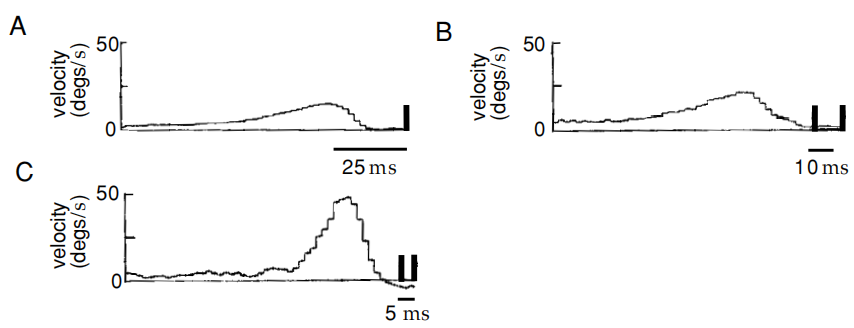
\includegraphics[scale=0.3]{./png/1.10-blowflyH1neuron.png}
    %figurecaption{Schematic of the procedure for computing the spike-triggered average stimulus. Each gray rectangle contains the stimulus prior to one of the spikes shown along the time axis. These are averaged to produce the waveform shown at the lower right, which is the average stimulus before a spike. The stimulus in this example is a piecewise constant function of time. (Adapted from Rieke et al.,1997.)}
    \label{fig:1.10}    
  \end{center}
\end{exm}
\begin{rem}
  Spike-triggered averages of other stimulus-dependent quantities can provide additional insight into neural encoding, for example, spike-triggered average autocorrelation functions. Obviously, spike-triggered averages of higher-order stimulus combinations can be considered as well.
\end{rem}

%%% Local Variables:
%%% mode: latex
%%% TeX-master: "../notesOnNeuroScience"
%%% End:
